% \newpage

\appendix

% 

\section{Dataset Examples}
\label{appx_data_examples}

We randomly select two data examples from each of the four datasets in our study (\S\ref{sec:data_models}), and present them in Table~\ref{tab:dataset_ex_1} and Table~\ref{tab:dataset_ex_2}.


\section{Details of Base LLMs}
\label{appx_model_details}

We provide brief descriptions for the 38 base LLMs adopted in this study in Table~\ref{tab:appx_model_registry}, discussed in \S\ref{sec:status-quo}.


%%%%%%%%%%%%%%%%%%%%%%%%%%%%%%%%%%%%%%%%%%%%%%%%%%%%%%
\section{Details of Evaluation Protocols}
\label{appx_prompts}

We provide a list of the 15 evaluation protocols investigated in this study in Table~\ref{tab:appx_method_registry}, detailed in \S\ref{sec:all_protocols}.
Below, we provide the prompt templates used for all prompting-based evaluation protocols in \S\ref{sec:all_protocols}.

\subsection{Prompt for Base Evaluation Protocol}
\label{appx_base_prompts}
Figure~\ref{fig:prompt_base} shows the prompt for the \texttt{base} protocol.
It corresponds to the \textit{Vanilla+Rules} prompting strategy proposed in \citet{{zeng2024evaluating}}.

\subsection{Prompts for Benchmark Evaluation Protocols}
\label{appx_benchmark_prompts}

We provide the prompts adopted from AlpacaEval~\cite{alpaca_eval} (Figure ~\ref{fig:prompt_alpaca}), ArenaHard~\cite{li2024crowdsourced} (Figure~ \ref{fig:prompt_arena}), and WildBench~\cite{lin2024wildbench}  (Figure~ \ref{fig:prompt_wildbench}).
The original evaluation protocols of ArenaHard and WildBench perform five-scale pairwise comparisons between the output pairs.
To better suit our task format, we modify their evaluation task to a binary pairwise comparison.
The evaluation protocol of WildBench requires a task-specific checklist of output quality to aid the evaluation.
In WildBench, these checklists were created using GPT-4-Turbo and Claude-3-Opus and manually reviewed.
Following a similar approach, we use GPT-4o to generate these checklists for the 4 datasets used in this work.

\subsection{Prompts for Enhanced Evaluation Protocols}
\label{appx_enhanced_prompts}

We list the prompts for \texttt{cot} (Figure~\ref{fig:prompt_cot}), \texttt{metric} (Figure~\ref{fig:prompt_metric_gen} \& Figure~\ref{fig:prompt_metric}), \texttt{reference} (Figure~\ref{fig:prompt_reference}), \texttt{metric+reference} (Figure~\ref{fig:prompt_metric_reference}), and \texttt{swap\&synthesize} (Figure~\ref{fig:prompt_swap_synthesis}).
These prompt templates are proposed by \citet{{zeng2024evaluating}}.


\subsection{Prompts for Complex Evaluation Protocols}
\label{appx_complex_prompts}
We present our prompts for \texttt{fine-grained-diff} (Figure~\ref{fig:prompt_finegrained_differences}), \texttt{multi-role-round2} (Figure~\ref{fig:prompt_multi-role_debate}), \texttt{multi-aspect-single} (Figure~\ref{fig:prompt_multi_aspect_one}), \texttt{multi-aspect-two} (Figure~\ref{fig:prompt_multi_aspect_two_analysis} and Figure~\ref{fig:prompt_multi_aspect_two_final}), \texttt{gpt4-reference} (Figure~\ref{fig:prompt_gpt4_reference}), and \texttt{prepair} (Figure~\ref{fig:prompt_prepair_pointwise} and Figure~\ref{fig:prompt_prepair_pairwise}).

% 


% 

\section{Case Study}
\label{appx_case_study}
We perform a qualitative analysis of the evaluation performance of \llama-3-70B and identify three main error patterns that impact its performance in various instances. The following paragraphs outline these error patterns, and we present a specific case study in Table~\ref{tab:appx_error_case}.

\paragraph{Surface-level deception \textsc{(surface)}} The model tends to favor outputs that appear more positive or have more structured presentations like numbered lists or professional layout despite clear disadvantages in addressing the instruction task compared to less structured but more appropriate and accurate responses. This failure mode is a recognized pattern across LLM-evaluators~\citep{zheng2024judging,wang-etal-2024-large-language-models-fair}.

\paragraph{Overlooking crucial context \textsc{(overlook)}} The model sometimes fails to identify important context in the question when it is not explicitly emphasized. This can lead to generic responses that miss key elements specific to the task at hand.

\paragraph{Counting issues \textsc{(counting)}} This applies to both numerical counting (for example, ``generate an 8-letter password'') and text-based context-relevant counting. The model often fails to count letters correctly or prefers longer outputs that exceed the instructed requirements, contrary to human annotators' preference for accurate answers.





\section{Generation Samples}
\label{appx_case_study_llama3_70b}
We present generation samples across different evaluation protocols of \llama-3-70B model for an example from \llmbarnatural, as shown in Figure~\ref{fig:appx_case_70b_data}. Model evaluations of \llama-3-70B under selected evaluation protocols are presented in Figure~\ref{fig:appx_case_70b_cot} (\texttt{cot}), Figure~\ref{fig:appx_case_70b_fine} (\texttt{fine-grained-diff}), Figure~\ref{fig:appx_case_70b_multi_role} (\texttt{multi-role-round2}),  and Figure~\ref{fig:appx_case_70b_prepair} (\texttt{prepair}).
Our analysis of the evaluation protocols reveals interesting disparities in their effectiveness. For example, the \texttt{cot} fails because it overlooks the factual error regarding the frequency of the word ``humans'' in one of the candidate outputs. In contrast, 
\texttt{multi-role-round2}'s success can be attributed to its multi-perspective debate approach, which allows for a more thorough examination and fact-checking of the claims made in each output.



%

%%%% all inputs
% 

\begin{table*}[ht]
  \centering
  \footnotesize
    \begin{tabular}{p{24.5em}c}
    \toprule
    \multicolumn{2}{l}{\textbf{\llmbarnatural}} \\
    \midrule
    \multicolumn{2}{l}{ Explain: Pathos, Ethos, Logos. } \\
    \midrule
    \multicolumn{1}{l}{\textbf{\lime{Output 1} }} & \multicolumn{1}{l}{\textbf{\red{Output 2} }} \\
   
Ethos is the ethical appeal, which is used to convince an audience of the author's credibility or character. 

Pathos is the emotional appeal, which is used to persuade an audience by appealing to their emotions. 

Logos is the appeal to logic and is used to convince an audience by the use of logic and reason.

& \multicolumn{1}{p{24.5em}}{Pathos is a tool of persuasion that is used to appeal to readers' emotions by arousing positive or negative feelings. 

It can be used in rhetoric, literature, film, and other forms of expression.

While pathos is used to draw an emotional response, the other rhetorical appeals appeal to credibility and logic, respectively.

Ethos is the distinguishing character, sentiment, moral nature, or guiding beliefs of a person, group, or institution. 

It is often evident as facts, numbers, or statistics and is used to convince an audience of an argument. } \\
    \midrule
    \multicolumn{2}{l}{\textbf{\adversarial}} \\
    \midrule
    \multicolumn{2}{l}{ Name an animal that is commonly kept as a pet.} \\
    \midrule
    \multicolumn{1}{l}{\textbf{\lime{Output 1}}} & \multicolumn{1}{l}{\textbf{\red{Output 2} }} \\
   
        Dogs are commonly kept as pets.
    & \multicolumn{1}{p{24.5em}}{Dogs, cats, and fish.} \\
    \midrule
    
    \multicolumn{2}{l}{\textbf{\mtbench}} \\
    \midrule
    \multicolumn{2}{l}{ A is the father of B. B is the father of C. What is the relationship between A and C?} \\
    \midrule
    \multicolumn{1}{l}{\textbf{\red{Output 1} }} & \multicolumn{1}{l}{\textbf{\lime{Output 2} }} \\
        A is the grandfather of C.
    & \multicolumn{1}{p{24.5em}}{

        * A is the father of B
        
        * B is the father of C
        
        * Therefore, A is the grandfather of C
        
        So the relationship between A and C is:
        
        Grandfather - Grandson

} \\

    \midrule
    \multicolumn{2}{l}{\textbf{\instrusum}} \\
    \midrule
\multicolumn{2}{l}{ % Use 1 column across, and left-align the text
    \parbox{13cm}{ % Set a paragraph box of width 12cm
         Here is an article:\\
        It is a book with 277 authors but with one shared experience - becoming a new mother in 2020.
        
        The mothers speak about their isolation, ...
        
        Please summarize the above article based on the given requirement:
    }
} \\
    \midrule
    \multicolumn{1}{l}{\textbf{\red{Output 1} }} & \multicolumn{1}{l}{\textbf{\lime{Output 2} }} \\
   
	    
Born in Lockdown is a book written by 277 new mothers in the UK about their experiences of becoming a mother during the pandemic. The mothers share their feelings of isolation, uncertainty, and pressure on their mental health, but also highlight the silver linings and positives that have come out of this joint experience. The project was set up by Bristol novelist Emylia Hall to encourage writing for pleasure and purpose. The book is an unflinchingly honest and moving account of new motherhood during the pandemic, where resilience, love, and hope shine through. The book is available for free download from the Mothership Writers website, with voluntary donations going to the stillbirth and neonatal death charity Sands.
& \multicolumn{1}{p{24.5em}}{Mothers in 2020 have experienced a unique set of challenges due to the pandemic, including isolation, uncertainty, and pressure on their mental health. Despite the hardships, many have found silver linings and positives that have come out of the shared experience. Through the writing project Born in Lockdown, 277 mothers from across the UK have shared their stories, expressing a range of emotions including resilience, love, and hope. } \\
    \bottomrule
    \end{tabular}%
  \caption{Selected examples from our datasets (\S\ref{sec:data_models}). The green label indicates the output is the preferred output.}
  \label{tab:dataset_ex_1}
\end{table*}%








 
\begin{table*}[t!]
  \centering
  \footnotesize
    \begin{tabular}{p{24.5em}c}
    \toprule
    \multicolumn{2}{l}{\textbf{\llmbarnatural}} \\
    \midrule
    \multicolumn{2}{l}{ 
    \parbox{13cm}{Given the following input statement, provide the type of sentiment in the statement and the extent of sentiment in terms of sentiment scores. This restaurant has the best service I've ever seen. You can design the score scale by yourself.}
    
    } \\
    \midrule
    \multicolumn{1}{l}{\textbf{\red{Output 1} }} & \multicolumn{1}{l}{\textbf{\lime{Output 2} }} \\
   
    This statement has a sentiment score of 9 / 10

& \multicolumn{1}{p{24.5em}}{Positive sentiment, sentiment score: 9.5 out of 10 } \\
    \midrule
    \multicolumn{2}{l}{\textbf{\adversarial}} \\
    \midrule
    \multicolumn{2}{l}{ Analyze the results of the following test scores. 90, 86, 75, 63} \\
    \midrule
    \multicolumn{1}{l}{\textbf{\red{Output 1}}} & \multicolumn{1}{l}{\textbf{\lime{Output 2} }} \\
   
        The average grade is 78.75.
    & \multicolumn{1}{p{24.5em}}{The test scores show a decreasing trend, with the first score being the highest and the last score being the lowest. This could indicate that the test taker's knowledge and skills were increasingly weak as the test progressed.} \\
    \midrule
    
    \multicolumn{2}{l}{\textbf{\mtbench}} \\
    \midrule
    \multicolumn{2}{l}{ 
    \parbox{15cm}{Identify the countries, their capitals, and the languages spoken in the following sentences. Output in JSON format.
    
    a) Amidst the idyllic vistas, Copenhagen, Denmark's capital, captivates visitors with its thriving art scene and the enchanting Danish language spoken by its inhabitants.
    
    b) Within the enchanting realm of Eldoria, one discovers Avalore, a grandiose city that emanates an ethereal aura. Lumina, a melodious language, serves as the principal mode of communication within this mystical abode.
    
    c) Nestled amidst a harmonious blend of age-old customs and contemporary wonders, Buenos Aires, the capital of Argentina, stands as a bustling metropolis. It is a vibrant hub where the expressive Spanish language holds sway over the city's inhabitants.}
    
    
    } \\
    \midrule
    \multicolumn{1}{l}{\textbf{\lime{Output 1} }} & \multicolumn{1}{l}{\textbf{\red{Output 2} }} \\
\{``sentences'': [

\{
``text'': ``Amidst the idyllic vistas, Copenhagen, Denmark's capital, captivates visitors with its thriving art scene and the enchanting Danish language spoken by its inhabitants.'',

``country'': ``Denmark'',

``capital'': ``Copenhagen'',

``language'': ``Danish''
\},

\{
``text'': ''Within the enchanting realm of Eldoria, one discovers Avalore, a grandiose city that emanates an ethereal aura. Lumina, a melodious language, serves as the principal mode of communication within this mystical abode.'',

``country'': ``Eldoria (fictional)'',

``capital'': ``Avalore (fictional)'',

``language'': ``Lumina (fictional)''
\},

\{
``text'': ``Nestled amidst a harmonious blend of age-old customs and contemporary wonders, Buenos Aires, the capital of Argentina, stands as a bustling metropolis. It is a vibrant hub where the expressive Spanish language holds sway over the city's inhabitants.'',

``country'': ``Argentina'',

``capital'': ``Buenos Aires'',

``language'': ``Spanish''
\}

]\}
    & \multicolumn{1}{p{24.5em}}{

    a) The capital of Denmark is Copenhagen. The language spoken in Denmark is Danish.
    
    b) The capital of Eldoria is Avalore. The language spoken in Eldoria is Lumina.
    
    c) The capital of Argentina is Buenos Aires. The language spoken in Argentina is Spanish.
 
} \\
\midrule
    \multicolumn{2}{l}{\textbf{\instrusum}} \\
    \midrule
    \multicolumn{2}{l}{ % Use 1 column across, and left-align the text
    \parbox{15cm}{ % Set a paragraph box of width 12cm
    Here is an article:
    
    As pressure to tackle London's housing crisis grows, a number of controversial views are being offered on how the problem...
    
    Please summarize the above article based on the given requirement:
    }
    } \\
    \midrule
    \multicolumn{1}{l}{\textbf{\lime{Output 1} }} & \multicolumn{1}{l}{\textbf{\red{Output 2} }} \\
   
Research director at The Adam Smith Institute, Sam Bowman, suggests that building on London's green belt lands could provide bigger and cheaper homes for everyone. However, Ann Goddard of Elstree \& Borehamwood Greenbelt Society argues that green belt lands are important for recreation purposes and to maintain a separation between settlements. Bowman proposes a compromise by differentiating between areas of beauty and intensive farmland within the green belt.

& \multicolumn{1}{p{24.5em}}{One solution to London's housing crisis is to build more properties on green belt lands. This would mean bigger and cheaper homes for everyone, but there is opposition to this idea as green belt land is seen as important for recreation and to make a demarcation between settlements. A compromise could be reached by differentiating between areas of beauty and intensive farmland.} \\
    \bottomrule
    \end{tabular}%
  \caption{Selected examples from our datasets (\S\ref{sec:data_models}). The green label indicates the output is the preferred output.}
  \label{tab:dataset_ex_2}
  
\end{table*}%




\begin{table*}[ht!]
    \centering
    \footnotesize
    \begin{tabular}{@{}lclc@{}}
    \toprule
    \multicolumn{1}{l}{\textbf{Name}} & \textbf{Size} & \textbf{License} & \multicolumn{1}{c}{\textbf{Description}} \\ \midrule
    \href{https://huggingface.co/google/gemma-2b-it}{gemma-2b}       & 2b  & Gemma & \multirow{2}{7cm}{Gemma is a family of open models from Google \citep{team2024gemma}}                       \\
    \href{https://huggingface.co/google/gemma-7b-it}{gemma-7b}       & 7b  & Gemma &                                          \\ \midrule
    \href{https://huggingface.co/THUDM/glm-4-9b-chat}{glm-4-9b}       & 9b  & GLM-4 & \parbox{7cm}{GLM-4-9B is an open-source version of the latest generation of pre-trained models launched by Zhipu AI~\citep{du2022glm}.}                                        \\ \midrule
    \href{https://huggingface.co/01-ai/Yi-1.5-9B-Chat}{yi-1.5-9b}       & 9b  & Yi & \multirow{2}{7cm}{Yi series are bilingual language models trained on a 3T multilingual corpus by 01.AI \citep{ai2024yi}}                       \\
    \href{https://huggingface.co/01-ai/Yi-1.5-34B-Chat}{yi-1.5-34b}       & 34b & Yi &                                          \\ \midrule
    \href{https://huggingface.co/meta-llama/Llama-2-7b-chat-hf}{llama-2-7b}       & 7b  & \llama 2 Community & \multirow{3}{7cm}{\llama 2 models are the latest generation developed by Meta AI \citep{touvron2023llama}, pretrained on 2.2T tokens.}                       \\
    \href{https://huggingface.co/meta-llama/Llama-2-13b-chat-hf}{llama-2-13b}       & 13b & \llama 2 Community &                                          \\
    \href{https://huggingface.co/meta-llama/Llama-2-70b-chat-hf}{llama-2-70b}       & 70b & \llama 2 Community &                                          \\
    \href{https://huggingface.co/meta-llama/Meta-Llama-3-8B-Instruct}{llama-3-8b}       & 8b  & \llama 3 Community & \multirow{2}{7cm}{\llama 3 are the latest open models from Meta AI \citep{meta_llama_3}, pretrained on 15T tokens.}                       \\
    \href{https://huggingface.co/meta-llama/Meta-Llama-3-70B-Instruct}{llama-3-70b}       & 70b & \llama 3 Community &                                          \\ 
    \href{https://huggingface.co/meta-llama/Meta-Llama-3.1-8B-Instruct}{llama-3.1-8b}       & 8b  & \llama 3.1 Community & \multirow{3}{7cm}{\llama 3.1 collection offers a series of multilingual models that outperform many open and closed chat models on industry benchmarks \citep{dubey2024llama}.}                       \\
    \href{https://huggingface.co/meta-llama/Meta-Llama-3.1-70B-Instruct}{llama-3.1-70b}       & 70b & \llama 3.1 Community &                                          \\
    \href{https://huggingface.co/meta-llama/Meta-Llama-3.1-405B-Instruct}{llama-3.1-405b}       & 405b & \llama 3.1 Community &                                          \\ \midrule 
    \href{https://huggingface.co/allenai/tulu-2-7b}{\tulu-2-7b}       & 7b  & AI2 ImpACT Low-risk & \multirow{6}{7cm}{\tulu V2 \citep{ivison2023camels} is a series of \llama 2 based models that are instruction-tuned on \tulumix.}                       \\
    \href{https://huggingface.co/allenai/tulu-2-dpo-7b}{\tulu-2-dpo-7b}       & 7b  & AI2 ImpACT Low-risk &                                          \\
    \href{https://huggingface.co/allenai/tulu-2-13b}{\tulu-2-13b}       & 13b & AI2 ImpACT Low-risk &                                          \\
    \href{https://huggingface.co/allenai/tulu-2-dpo-13b}{\tulu-2-dpo-13b}       & 13b & AI2 ImpACT Low-risk &                                          \\
    \href{https://huggingface.co/allenai/tulu-2-70b}{\tulu-2-70b}       & 70b & AI2 ImpACT Low-risk &                                          \\
    \href{https://huggingface.co/allenai/tulu-2-dpo-70b}{\tulu-2-dpo-70b}       & 70b & AI2 ImpACT Low-risk &                                          \\ \midrule
    \href{https://deepmind.google/technologies/gemini/}{gemini-1.0-pro}       & -             & Proprietary & \multirow{3}{7cm}{Gemini models are the most capable multimodal models from Google featuring long context lengths \citep{team2023gemini}.}                       \\
    \href{https://deepmind.google/technologies/gemini/}{gemini-1.5-flash}       & -             & Proprietary &                                          \\
    \href{https://deepmind.google/technologies/gemini/}{gemini-1.5-pro}       & -             & Proprietary &                                          \\ \midrule
    \href{https://huggingface.co/Qwen/Qwen1.5-32B-Chat}{qwen-1.5-32b}       & 32b  & Qianwen & \multirow{4}{7cm}{Qwen is a family of models built by Alibaba Cloud~\citep{qwen}. Qwen1.5 and Qwen2 have recently surpassed most open models on common benchmarks.}                       \\
    \href{https://huggingface.co/Qwen/Qwen1.5-72B-Chat}{qwen-1.5-72b}       & 72b  & Qianwen &                                          \\
    \href{https://huggingface.co/Qwen/Qwen2-72B-Instruct}{qwen-2-72b}       & 72b  & Qianwen &                                          \\
    \href{https://huggingface.co/Qwen/Qwen2.5-72B-Instruct}{qwen-2.5-72b}       & 72b  & Qianwen &                                          \\
        \midrule
    \href{https://huggingface.co/mistralai/Mistral-7B-Instruct-v0.3}{mistral-7b-v0.3}          & 7b  & Apache 2.0 & \multirow{2}{7cm}{Instruction-tuned versions of Mistral models~\citep{jiang2023mistral} from Mistral AI.}                       \\
    % \href{https://huggingface.co/mistralai/Mistral-7B-Instruct-v0.2}{mistral-7b-v0.2}       & 7b  & Apache 2.0 &                                          \\
    % \href{https://huggingface.co/mistralai/Mistral-7B-Instruct-v0.3}{mistral-7b-v0.3}       & 7b  & Apache 2.0 &                                          \\
    \href{https://mistral.ai/news/mistral-large/}{mistral-large}       & -             & Proprietary &                                          \\ \midrule
    \href{https://huggingface.co/mistralai/Mixtral-8x7B-Instruct-v0.1}{mixtral-8x7b}       & 8x7b & Apache 2.0 & \parbox{7cm}{Mixtral-8x22B is a pretrained generative Sparse Mixture of Experts (MoE) from Mistral AI~\citep{jiang2024mixtral}}                                        \\ \midrule
    \href{https://www.anthropic.com/api}{claude-3-haiku}       & -             & Proprietary & \multirow{3}{7cm}{Claude-3-Haiku and Claude 3 Opus, and Claude 3.5 Sonnet are top proprietary models trained by Anthropic PBC \citep{claude}.}                       \\
    \href{https://www.anthropic.com/api}{claude-3-opus}       & -             & Proprietary &                                          \\
     \href{https://www.anthropic.com/api}{claude-3.5-sonnet}       & -             & Proprietary &                                          \\
        \midrule
    \href{https://platform.openai.com/docs/models}{gpt-3.5-turbo-0125}       & -             & Proprietary & \multirow{3}{7cm}{GPT models are strong proprietary models~\citep{achiam2023gpt} from OpenAI. ``o1'' model was released in September 2024 with strong reasoning capability. }                       \\
             \href{https://platform.openai.com/docs/models}{gpt-4-0613}                   & -             & Proprietary & \\

    \href{https://platform.openai.com/docs/models}{gpt-4o-2024-05-13}                   & -             & Proprietary & \\
     \href{https://platform.openai.com/docs/models}{gpt-4o-2024-08-06}                   & -             & Proprietary & \\
  \href{https://platform.openai.com/docs/models}{o1-mini-2024-0912}                   & -             & Proprietary & \\
 \midrule
    \href{https://huggingface.co/prometheus-eval/prometheus-8x7b-v2.0}{prometheus-2-8x7b}       & 8x7b  & Apache 2.0 & \parbox{7cm}{Prometheus 2 is an alternative to GPT-4 for fine-grained evaluation of LLMs and reward models for RLHF, based on Mistral-Instruct~\citep{kim2024prometheus2}}                                        \\ 
    \href{https://huggingface.co/NCSOFT/Llama-3-OffsetBias-8B}{offsetbias-lm}       & 8b  & \llama 3 Community & \parbox{7cm}{OffsetBias is a generative judge model for pairwise preference evaluation, designed to be robust against various evaluation biases~\citep{park2024offsetbias}}                                        \\ \midrule
    
  \href{https://huggingface.co/nvidia/Nemotron-4-340B-Reward}{nemotron-4-340b-reward}       & 340b  & NVIDIA Open Model & \parbox{7cm}{A multi-aspect reward model for synthetic data generation and RLAIF, based on Nemotron-4-340B-Base~\citep{wang2024helpsteer2}}   \\                                
    \href{https://huggingface.co/NCSOFT/Llama-3-OffsetBias-RM-8B}{offsetbias-rm}       & 8b  & \llama 3 Community & \parbox{7cm}{Reward model trained on OffsetBias dataset, designed to be robust against various evaluation biases~\citep{park2024offsetbias}}                                        \\ 

     \bottomrule
    \end{tabular}
    \caption{Model registry and metadata in our study used in \S\ref{sec:status-quo}.}
    \label{tab:appx_model_registry}
    \end{table*}
\begin{table*}[ht!]
    \centering
    \footnotesize
    \begin{tabular}{@{}lll@{}}
    \toprule
    \textbf{Full Name} & \textbf{Code Name} & \textbf{Related Work} \\
    \midrule
    Base Pairwise Evaluation & base & \citet{zeng2024evaluating} \\
    Chain-of-Thought & cot & \citet{zeng2024evaluating,wei2022chain} \\
    Metric Generation & metric & \citet{zeng2024evaluating} \\
    Reference Generation & reference & \citet{zeng2024evaluating}  \\
    Metric and Reference & metric+reference & \citet{zeng2024evaluating} \\
    Swap and Synthesize & swap\&synthesize  & \citet{zeng2024evaluating} \\
    Fine-grained Differences & fine-grained-diff & Inspired by \citet{liu-etal-2023-revisiting, liu-etal-2023-towards-interpretable, min-etal-2023-factscore} \\
    Multi-Role Debate (Single Round) & multi-role-round1  & \citet{chan2024chateval} \\
    Multi-Role Debate (Two Rounds) & multi-role-round2  & \citet{chan2024chateval} \\
    Multi-Aspect Comparison (Two-Stage) & multi-aspect-two  & \citet{li2024decompose} \\
    Multi-Aspect Comparison (Single-Stage) & multi-aspect-single  & \citet{li2024decompose} \\
    GPT-4 Reference & gpt4-reference & Modified from \citet{zeng2024evaluating} \\
    Pointwise Reasoning Enhanced Pairwise & prepair  & \citet{jeong2024prepair} \\
    Self-Consistency over CoTs & cot\&consistency & \citet{wang2023selfconsistency} \\
    Self-Consistency over Different Protocols & protocol-consistency & \citet{wang2023selfconsistency} \\
    \bottomrule
    \end{tabular}
    \caption{Method registry for evaluation protocols in \S\ref{sec:all_protocols}}
    \label{tab:appx_method_registry}
\end{table*}
\clearpage
\begin{figure*}[t!]
\begin{tcolorbox}[colback=black!3!white, colframe=black!70!white, title=Base, fontupper=\footnotesize, fonttitle=\footnotesize]
\textbf{[System Message]} \\
You are a helpful assistant in evaluating the quality of the outputs for a given instruction. Your goal is to select the best output for the given instruction.
\newline
\newline
\textbf{[User Message]}\\
Select the Output (a) or Output (b) that is better for the given instruction. The two outputs are generated by two different AI chatbots respectively. \\
\newline
Here are some rules of the evaluation: \\
(1) You should prioritize evaluating whether the output honestly/precisely/closely executes the instruction, then consider its helpfulness, accuracy, level of detail, harmlessness, etc. \\
(2) Outputs should NOT contain more/less than what the instruction asks for, as such outputs do NOT precisely execute the instruction.\\
(3) You should avoid any potential bias and your judgment should be as objective as possible. For example, the order in which the outputs were presented should NOT affect your judgment, as Output (a) and Output (b) are equally likely to be the better.
\newline
\newline
Do NOT provide any explanation for your choice.\\
Do NOT say both / neither are good.\\
You should answer using ONLY "Output (a)" or "Output (b)". Do NOT output any other words.\\
\newline

\# Instruction: \\
\{INSTRUCTION\}
\newline
\newline
\# Output (a): \\
\{OUTPUT\_1\}
\newline
\newline
\# Output (b): \\
\{OUTPUT\_2\}
\newline
\newline
\# Which is better, Output (a) or Output (b)? Your response should be either "Output (a)" or "Output (b)":
\end{tcolorbox}
\caption{Prompt for \texttt{base} protocol described in \S\ref{sec:all_protocols}.}
\label{fig:prompt_base}
\end{figure*}


\begin{figure*}[t!]
\begin{tcolorbox}[colback=black!3!white, colframe=black!70!white, title=AlpacaEval, fontupper=\footnotesize, fonttitle=\footnotesize]
\textbf{[System Message]} \\
You are a highly efficient assistant, who evaluates and selects the best large language model (LLMs) based on the quality of their responses to a given instruction. This process will be used to create a leaderboard reflecting the most accurate and human-preferred answers.
\newline
\newline
\textbf{[User Message]}\\
I require a leaderboard for various large language models. I'll provide you with prompts given to these models and their corresponding outputs. Your task is to assess these responses, and select the model that produces the best output from a human perspective. \\
\newline

\#\# Instruction

\{ \\
    "instruction": """\{INSTRUCTION\}""",\\
\}\\
\newline
\newline
\#\# Model Outputs
\newline

Here are the unordered outputs from the models. Each output is associated with a specific model, identified by a unique model identifier.
\\
\{\\
\hspace*{1cm}  \{
        "model\_identifier":  "m",\\
         \hspace*{1cm} "output": """\{OUTPUT\_1\}"""\\
   \hspace*{1cm}  \},\\
    \hspace*{1cm}\{\\
       \hspace*{1cm} "model\_identifier": "M",\\
        \hspace*{1cm}"output": """\{OUTPUT\_2\}"""\\
   \hspace*{1cm}       \}\\
\}\\
\newline
\#\# Task
\newline
Evaluate the models based on the quality and relevance of their outputs, and select the model that generated the best output. Answer by providing the model identifier of the best model. We will use your output as the name of the best model, so make sure your output only contains one of the following model identifiers and nothing else (no quotes, no spaces, no new lines, ...): Model (m) or Model (M).
\\ 

\#\# Which is better, Model (m) or Model (M)? Your response should be either "Model (m)" or "Model (M)":
\end{tcolorbox}
\caption{Prompt for AlpacaEval baseline described in \S\ref{baselines_protocols}}
\label{fig:prompt_alpaca}
\end{figure*}



\begin{figure*}[t!]
\begin{tcolorbox}[colback=black!3!white, colframe=black!70!white, title=ArenaHard, fontupper=\footnotesize, fonttitle=\footnotesize]
\textbf{[System Message]} \\
Please act as an impartial judge and evaluate the quality of the responses provided by two AI assistants to the user prompt displayed below. You will be given assistant A's answer and assistant B's answer. Your job is to evaluate which assistant's answer is better.
\newline
\textbf{[User Message]}\\
Begin your evaluation by generating your own answer to the prompt. You must provide your answers before judging any answers.
\newline

When evaluating the assistants' answers, compare both assistants' answers with your answer. You must identify and correct any mistakes or inaccurate information.
\newline


Then consider if the assistant's answers are helpful, relevant, and concise. Helpful means the answer correctly responds to the prompt or follows the instructions. Note when user prompt has any ambiguity or more than one interpretation, it is more helpful and appropriate to ask for clarifications or more information from the user than providing an answer based on assumptions. Relevant means all parts of the response closely connect or are appropriate to what is being asked. Concise means the response is clear and not verbose or excessive.
\newline

Then consider the creativity and novelty of the assistant's answers when needed. Finally, identify any missing important information in the assistants' answers that would be beneficial to include when responding to the user prompt.
\newline

After providing your explanation, you must always end your response with either "Therefore, Answer (a) is better." or "Therefore, Answer (b) is better." verbatim.
\newline
\newline

<|User Prompt|>\\
\{INSTRUCTION\}
\\ 
\\
<|The Start of Answer (a)|> \\
\{OUTPUT\_1\} \\
<|The End of Answer (a)|>
\\
\\
<|The Start of Answer (b)|> \\
\{OUTPUT\_2\}\\
<|The End of Answer(b)|>\\
\\

\# Decision (Give an explanation of your evaluation followed by either "Therefore, Answer (a) is better." or "Therefore, Answer (b) is better." verbatim. Always claim which is better at the end.):

\end{tcolorbox}
\caption{Prompt for ArenaHard described in \S\ref{baselines_protocols}}
\label{fig:prompt_arena}
\end{figure*}




\begin{figure*}[t!]
\begin{tcolorbox}[colback=black!3!white, colframe=black!70!white, title=WildBench, fontupper=\footnotesize, fonttitle=\footnotesize]
\textbf{[System Message]} \\
You are an expert evaluator. Your task is to evaluate the quality of the responses generated by two AI models. 
\newline
\textbf{[User Message]}\\
\# Instruction 
\\ \\ 
We will provide you with the user query and a pair of AI-generated responses (Response A and Response B). \\
You should first read the user query and the conversation history carefully for analyzing the task, and then evaluate the quality of the responses based on and rules provided below. \\
\newline

\# Conversation between User and AI
\\ 
\#\# User Query \\
<|begin\_of\_query|> \\
\{INSTRUCTION\} \\
<|end\_of\_query|>
\\ \\
\#\# Response A \\
<|begin\_of\_response\_A|> \\
\{OUTPUT\_1\}
\newline
<|end\_of\_response\_A|> \\

\#\# Response B \\
<|begin\_of\_response\_B|> \\
\{OUTPUT\_2\}
\\
<|end\_of\_response\_B|>
\\
\\
\# Evaluation   
\\ 
\#\# Checklist 
\newline
<|begin\_of\_checklist|> \\
\{CHECKLIST\} \\
<|end\_of\_checklist|> \\
\newline

Please use this checklist to guide your evaluation, but do not limit your assessment to the checklist.
\\
\\ 

\#\# Rules 
\newline
\newline
You should compare the above two responses based on your analysis of the user query. \\
You should first write down your analysis and the checklist that you used for the evaluation, and then provide your assessment according to the checklist. \\
You should always end your response by selecting the better response. \\
\newline

\#\# Output Format \\

First, please output your analysis for each model response, and then summarize your assessment to three aspects: "reason A=B", "reason A>B", and "reason B>A", and finally make your choice for the final assessment by selecting the better response (ties are NOT allowed). \\
\newline
Please provide your evaluation results in the following json format by filling in the placeholders in []: \\

``` \\
\{ \\
\hspace*{1cm} "analysis of A": "[analysis of Response A]", \\
  \hspace*{1cm}  "analysis of B": "[analysis of Response B]",\\
  \hspace*{1cm}  "reason of A=B": "[where Response A and B perform equally well]", \\
  \hspace*{1cm}  "reason of A>B": "[where Response A is better than Response B]", \\
  \hspace*{1cm}  "reason of B>A": "[where Response B is better than Response A]", \\
  \hspace*{1cm}  "choice": "[Response (A) or Response (B)]", \\
\} \\
```


\end{tcolorbox}
\caption{Prompt for WildBench baseline described in \S\ref{baselines_protocols}}
\label{fig:prompt_wildbench}
\end{figure*}

\begin{figure*}[t!]
\begin{tcolorbox}[colback=black!3!white, colframe=black!70!white, title=CoT, fontupper=\footnotesize, fonttitle=\footnotesize]
\textbf{[System Message]} \\
You are a helpful assistant in evaluating the quality of the outputs for a given instruction. Your goal is to select the best output for the given instruction.
\newline
\newline
\textbf{[User Message]}\\
After giving a brief explanation, select the Output (a) or Output (b) that is better for the given instruction. The two outputs are generated by two different AI chatbots respectively.
\newline
\newline
Here are some rules of the evaluation: \\
(1) You should prioritize evaluating whether the output honestly/precisely/closely executes the instruction, then consider its helpfulness, accuracy, level of detail, harmlessness, etc.\\
(2) Outputs should NOT contain more/less than what the instruction asks for, as such outputs do NOT precisely execute the instruction. \\
(3) You should avoid any potential bias and your judgment should be as objective as possible. For example, the order in which the outputs were presented should NOT affect your judgment, as Output (a) and Output (b) are equally likely to be the better.\\
\newline
\newline
You should first provide a brief explanation of your evaluation, and then always end your response with either "Therefore, Output (a) is better." or "Therefore, Output (b) is better." verbatim.\\
Do NOT say both / neither are good.\\
Do NOT output any other words.\\
Do NOT say "Output (a) is better" or "Output (b) is better" at the beginning. You should do reasoning and thinking before claiming which is better.\\
\newline
\# Instruction: \\
\{INSTRUCTION\}
\newline
\newline
\# Output (a): \\
\{OUTPUT\_1\}
\newline
\newline
\# Output (b): \\
\{OUTPUT\_2\}
\newline
\newline
\# Decision (Give a brief explanation of your evaluation followed by either "Therefore, Output (a) is better." or "Therefore, Output (b) is better." verbatim. Always claim which is better at the end. In your explanation, you should always use "Output (a)" or "Output (b)" to refer to the two outputs respectively.):
\end{tcolorbox}
\caption{Prompt for \texttt{cot} protocol described in \S\ref{sec:all_protocols}.}
\label{fig:prompt_cot}
\end{figure*}




\begin{figure*}[t!]
\begin{tcolorbox}[colback=black!3!white, colframe=black!70!white, title=Metric (metric generation prompt), fontupper=\footnotesize, fonttitle=\footnotesize]
\textbf{[System Message]} \\
You are a helpful assistant.
\newline
\newline
\textbf{[User Message]}\\
Please propose at most three concise questions about whether a potential output is a good output for a given instruction. Another assistant will evaluate different aspects of the output by answering all the questions.
\newline
\newline
Here are some rules of the evaluation: \\
(1) You should prioritize evaluating whether the output honestly/precisely/closely executes the instruction.
\\
(2) Outputs should NOT contain more/less than what the instruction asks for, as such outputs do NOT precisely execute the instruction.
\\
\newline
\# Instruction: \\
\{INSTRUCTION\}
\newline
\newline
\# Requirements for Your Output: \\
(1) The questions should **specifically** target the given instruction instead of some general standards, so the questions may revolve around key points of the instruction. \\
(2) You should directly give the questions without any other words. \\
(3) Questions are presented from most important to least important.\\
\newline
\# Please give your questions here:

\end{tcolorbox}
\caption{Prompt for metric generation stage of the \texttt{metric} protocol described in \S\ref{sec:all_protocols}.}
\label{fig:prompt_metric_gen}
\end{figure*}



\begin{figure*}[t!]
\begin{tcolorbox}[colback=black!3!white, colframe=black!70!white, title=Metric, fontupper=\footnotesize, fonttitle=\footnotesize]
\textbf{[System Message]} \\
You are a helpful assistant in evaluating the quality of the outputs for a given instruction. Your goal is to select the best output for the given instruction.
\newline
\newline
\textbf{[User Message]}\\
Select the Output (a) or Output (b) that is better for the given instruction. The two outputs are generated by two different AI chatbots respectively.
\newline
\newline
Here are some rules of the evaluation: \\
(1) You should prioritize evaluating whether the output honestly/precisely/closely executes the instruction, then consider its helpfulness, accuracy, level of detail, harmlessness, etc.\\
(2) Outputs should NOT contain more/less than what the instruction asks for, as such outputs do NOT precisely execute the instruction.\\
(3) You should avoid any potential bias and your judgment should be as objective as possible. For example, the order in which the outputs were presented should NOT affect your judgment, as Output (a) and Output (b) are equally likely to be the better.\\
\newline
\newline
Do NOT provide any explanation for your choice. \\
Do NOT say both / neither are good.\\
You should answer using ONLY "Output (a)" or "Output (b)". Do NOT output any other words.\\
\newline
\newline
\# Instruction: \\
\{INSTRUCTION\}
\newline
\newline
\# Output (a): \\
\{OUTPUT\_1\}
\newline
\newline
\# Output (b): \\
\{OUTPUT\_2\}
\newline
\newline
\# Questions about Outputs:\\
Here are at most three questions about the outputs, which are presented from most important to least important. You can do the evaluation based on thinking about all the questions. \\
\{QUESTIONS\}
\newline
\newline
\# Which is better, Output (a) or Output (b)? Your response should be either "Output (a)" or "Output (b)":
\end{tcolorbox}
\caption{Prompt for \texttt{metric} protocol described in \S\ref{sec:all_protocols}.}
\label{fig:prompt_metric}
\end{figure*}


\begin{figure*}[t!]
\begin{tcolorbox}[colback=black!3!white, colframe=black!70!white, title=Reference, fontupper=\footnotesize, fonttitle=\footnotesize]
\textbf{[System Message]} \\
You are a helpful assistant in evaluating the quality of the outputs for a given instruction. Your goal is to select the best output for the given instruction.
\newline
\newline
\textbf{[User Message]}\\
Select the Output (a) or Output (b) that is better for the given instruction. The two outputs are generated by two different AI chatbots respectively.
\newline\newline
Here are some rules of the evaluation:
\newline
(1) You should prioritize evaluating whether the output honestly/precisely/closely executes the instruction, then consider its helpfulness, accuracy, level of detail, harmlessness, etc.\\
(2) Outputs should NOT contain more/less than what the instruction asks for, as such outputs do NOT precisely execute the instruction.\\
(3) You should avoid any potential bias and your judgment should be as objective as possible. For example, the order in which the outputs were presented should NOT affect your judgment, as Output (a) and Output (b) are equally likely to be the better.\\
\newline
\newline
Do NOT provide any explanation for your choice. \\
Do NOT say both / neither are good.\\
You should answer using ONLY "Output (a)" or "Output (b)". Do NOT output any other words.\\
\newline
\newline
\# Instruction: \\
\{INSTRUCTION\}
\newline\newline
\# Output (a): \\
\{OUTPUT\_1\}
\newline\newline
\# Output (b):\\
\{OUTPUT\_2\}
\newline\newline
\# A reference output generated by a strong AI assistant: \\
\{REFERENCE\}
\newline
\newline
\# Which is better, Output (a) or Output (b)? Your response should be either "Output (a)" or "Output (b)":
\end{tcolorbox}
\caption{Prompt for \texttt{reference} protocol described in \S\ref{sec:all_protocols}.}
\label{fig:prompt_reference}
\end{figure*}


\begin{figure*}[t!]
\begin{tcolorbox}[colback=black!3!white, colframe=black!70!white, title=Metric + Reference, fontupper=\footnotesize, fonttitle=\footnotesize]
\textbf{[System Message]} \\
You are a helpful assistant in evaluating the quality of the outputs for a given instruction. Your goal is to select the best output for the given instruction.
\newline

\textbf{[User Message]}\\
Select the Output (a) or Output (b) that is better for the given instruction. The two outputs are generated by two different AI chatbots respectively.
\newline

Here are some rules of the evaluation:

(1) You should prioritize evaluating whether the output honestly/precisely/closely executes the instruction, then consider its helpfulness, accuracy, level of detail, harmlessness, etc.

(2) Outputs should NOT contain more/less than what the instruction asks for, as such outputs do NOT precisely execute the instruction.

(3) You should avoid any potential bias and your judgment should be as objective as possible. For example, the order in which the outputs were presented should NOT affect your judgment, as Output (a) and Output (b) are equally likely to be the better.
\newline

Do NOT provide any explanation for your choice. \\
Do NOT say both / neither are good. \\
You should answer using ONLY "Output (a)" or "Output (b)". Do NOT output any other words.\\

\# Instruction:

\{INSTRUCTION\}
\newline

\# Output (a):

\{OUTPUT\_1\}
\newline

\# Output (b):

\{OUTPUT\_2\}
\newline

\# Questions about Outputs:

Here are at most three questions about the outputs, which are presented from most important to least important. You can do the evaluation based on thinking about all the questions.

\{QUESTIONS\}
\newline

\# A reference output generated by a strong AI assistant:

\{REFERENCE\}
\newline

\# Which is better, Output (a) or Output (b)? Your response should be either "Output (a)" or "Output (b)":
\end{tcolorbox}
\caption{Prompt for \texttt{metric + reference} protocol described in \S\ref{sec:all_protocols}.}
\label{fig:prompt_metric_reference}
\end{figure*}




\begin{figure*}[t!]
\begin{tcolorbox}[colback=black!3!white, colframe=black!70!white, title=Swap\&Synthesize, fontupper=\footnotesize, fonttitle=\footnotesize]
\textbf{[System Message]} \\
You are a helpful assistant who reviews a debate between two other assistants in evaluating the quality of the outputs for a given instruction.
\newline

\textbf{[User Message]}\\
The two assistants, Assistant (a) and Assistant (b), are given an instruction, Output (a) and Output (b). They are asked to select the Output (a) or Output (b) that is better for the given instruction. Output (a) and Output (b) are generated by two different AI chatbots respectively.
\newline


Assistant (a) and Assistant (b) have conflicting evaluations. Your goal is to review their evaluations and give your final decision on which output is better.
\newline

Here are some rules of the evaluation:

(1) You should prioritize evaluating whether the output honestly/precisely/closely executes the instruction, then consider its helpfulness, accuracy, level of detail, harmlessness, etc.

(2) Outputs should NOT contain more/less than what the instruction asks for, as such outputs do NOT precisely execute the instruction.

(3) You should avoid any potential bias and your judgment should be as objective as possible. For example, the order in which the outputs were presented should NOT affect your judgment, as Output (a) and Output (b) are equally likely to be the better.
\newline

Now carefully review the instruction, Output (a), Output (b), and the debate between Assistant (a) and Assistant (b). Select the Output (a) or Output (b) that is better for the given instruction.

Do NOT provide any explanation for your choice.

Do NOT say both / neither are good.

You should answer using ONLY "Output (a)" or "Output (b)". Do NOT output any other words.
\newline

\# Instruction:

\{INSTRUCTION\}\newline

\# Output (b):

\{OUTPUT\_2\}\newline

\# Output (a):

\{OUTPUT\_1\}\newline


\# Debate between Assistant (a) and Assistant (b): 

\#\# Evaluation given by Assistant (a), who thinks Output (a) is better:

\{EXPLANATION\_1\}

\#\# Evaluation given by Assistant (b), who thinks Output (b) is better:

\{EXPLANATION\_2\}
\newline

\# Which is better, Output (a) or Output (b)? Your response should be either "Output (a)" or "Output (b)":
\end{tcolorbox}
\caption{Prompt for \texttt{swap\&synthesize} protocol described in \S\ref{sec:all_protocols}.}
\label{fig:prompt_swap_synthesis}
\end{figure*}




\begin{figure*}[t!]
\begin{tcolorbox}[colback=black!3!white, colframe=black!70!white, title=Fine-grained-diff, fontupper=\footnotesize, fonttitle=\footnotesize]
\textbf{[System Message]} \\
You are a helpful assistant in evaluating the quality of the outputs for a given instruction. Your goal is to select the best output for the given instruction.
\newline
\newline
\textbf{[User Message]}\\
After giving a detailed explanation, select either Output (a) or Output (b) as the better response for the given instruction. The two outputs are generated by two different AI chatbots respectively.
\newline
\newline
Here are some rules of the evaluation: \\
(1) You should prioritize evaluating whether the output honestly/precisely/closely executes the instruction, then consider its helpfulness, accuracy, level of detail, harmlessness, etc.\\
(2) Outputs should NOT contain more/less than what the instruction asks for, as such outputs do NOT precisely execute the instruction.\\
(3) You should avoid any potential bias and your judgment should be as objective as possible. For example, the order in which the outputs were presented should NOT affect your judgment, as Output (a) and Output (b) are equally likely to be the better.\\
\newline
You should first provide a detailed explanation of your evaluation, and then always end your response with either "Therefore, Output (a) is better." or "Therefore, Output (b) is better." verbatim.\\
Do NOT say both / neither are good.\\
Do NOT output any other words.\\
Do NOT say "Output (a) is better" or "Output (b) is better" at the beginning. You should do reasoning and thinking before claiming which is better.\\
\newline
Here is the evaluation plan:

1. Differences Identification: Enumerate the key fine-grained content differences observed between Output (a) and Output (b).\\
2. Explanation and Rationale: Provide explanations and rationale for which output better addresses the instruction by considering these differences, as well as other relevant factors such as relevance, completeness, coherence, and clarity.\\
3. Final Decision: End your response with either "Therefore, Output (a) is better." or "Therefore, Output (b) is better." verbatim.\\
\newline
Provide your response in the following format:\\
"""\\
Differences Identification: \\
\newline
1. [Difference 1] \\
2. [Difference 2] \\
... \\
N. [Difference N] \\
\newline
Explanation and Rationale: [Detailed explanation and rationale for your decision] \\

Final Decision: Therefore, Output (a)/Output (b) is better. \\
"""\\

\# Instruction: \\
\{INSTRUCTION\}
\newline
\newline
\# Output (a): \\
\{OUTPUT\_1\}
\newline
\newline
\# Output (b): \\
\{OUTPUT\_2\}
\newline

\# Your Response (Give a detailed explanation of your evaluation followed by either "Therefore, Output (a) is better." or "Therefore, Output (b) is better." verbatim. Always claim which is better at the end. In your explanation, you should always use "Output (a)" or "Output (b)" to refer to the two outputs respectively.):

\end{tcolorbox}
\caption{Prompt for \texttt{fine-graine-diff} protocol described in \S\ref{sec:all_protocols}.}
\label{fig:prompt_finegrained_differences}
\end{figure*}





\begin{figure*}[t!]
\begin{tcolorbox}[colback=black!3!white, colframe=black!70!white, title=Multi-role-round2, fontupper=\footnotesize, fonttitle=\footnotesize]
\textbf{[System Message]} \\
You are a helpful assistant who evaluates the quality of the outputs for a given instruction. Your goal is to select the best output for the given instruction.
\newline

\textbf{[User Message]}\\
Select the Output (a) or Output (b) that is better for the given instruction. The two outputs are generated by two different AI chatbots respectively.
\newline

Here are some rules of the evaluation:

(1) You should prioritize evaluating whether the output honestly/precisely/closely executes the instruction, then consider its helpfulness, accuracy, level of detail, harmlessness, etc.

(2) Outputs should NOT contain more/less than what the instruction asks for, as such outputs do NOT precisely execute the instruction.

(3) You should avoid any potential bias and your judgment should be as objective as possible. For example, the order in which the outputs were presented should NOT affect your judgment, as Output (a) and Output (b) are equally likely to be the better.
\newline

You should first provide a brief explanation of your evaluation, and then always end your response with either "Therefore, Output (a) is better." or "Therefore, Output (b) is better." verbatim.

Do NOT say both / neither are good.

Do NOT output any other words.

Do NOT say "Output (a) is better" or "Output (b) is better" at the beginning. You should do reasoning and thinking before claiming which is better.
\newline

There are a few other referees assigned the same task, it's your responsibility to discuss with them and think critically before you make your final judgement. You should avoid any potential bias and ensure that the order in which the responses were presented does not affect your judgment. Debate with others.

Always end your response with "Therefore, Output (a) is better." or "Therefore, Output (b) is better." verbatim. Make sure to make the claim to end your response.
\newline

\# Instruction: \\
\{INSTRUCTION\}
\newline

\# Output (a): \\
\{OUTPUT\_1\}
\newline

\# Output (b): \\
\{OUTPUT\_2\}
\newline

\# Previous referees' arguments: \\
\{CHAT\_HISTORY\}
\newline

\# Your role:

\{ROLE\_DESCRIPTION\}
\newline

\# Decision (Give a brief explanation of your evaluation followed by either "Therefore, Output (a) is better." or "Therefore, Output (b) is better." verbatim. Always claim which is better at the end. In your explanation, you should always use "Output (a)" or "Output (b)" to refer to the two outputs respectively.):
\end{tcolorbox}
\caption{Prompt for \texttt{Multi-role-round2} protocol described in \S\ref{sec:all_protocols}.}
\label{fig:prompt_multi-role_debate}
\end{figure*}





\begin{figure*}[t!]
\begin{tcolorbox}[colback=black!3!white, colframe=black!70!white, title=Multi-aspect-single, fontupper=\scriptsize, fonttitle=\footnotesize]
\textbf{[System Message]} \\
You are a helpful assistant who analyzes and evaluates the quality of two candidate outputs for a given instruction task based on a list of criteria, and makes a final decision on which output is better.
\newline

\textbf{[User Message]}\\
Given an instruction and two responses, Output (a) and Output (b), each aiming to fulfill the task, your task is to carefully analyze and evaluate each output based on a list of criteria.
\newline

Here are some general rules for the evaluation:

(1) You should prioritize evaluating whether the output honestly/precisely/closely executes the instruction, then consider its helpfulness, accuracy, level of detail, harmlessness, etc.

(2) Outputs should NOT contain more or less than what the instruction asks for, as such outputs do NOT precisely execute the instruction.
(3) You should avoid any potential bias and your judgment should be as objective as possible. For example, the order in which the outputs were presented should NOT affect your judgment, as Output (a) and Output (b) are equally likely to be the better one.
\newline

You should first provide an explanation of your evaluation, and then always end your response with either "Therefore, Output (a) is better." or "Therefore, Output (b) is better." verbatim.

Do NOT say both / neither are good.

Do NOT output any other words.

Do NOT say "Output (a) is better" or "Output (b) is better" at the beginning. You should do reasoning and thinking before claiming which output is better.
\newline

Here are some criteria to consider:

1. Text Quality: The response should be fluent, well-structured, and free of spelling and grammatical errors. It should also be coherent, with a clear and logical flow of ideas.

2. Information Richness: The response is encouraged to provide rich, detailed and professional information, e.g. by providing examples, explanations, citations, and additional information. This criterion is not applicable if the user asks for a short or direct answer without additional information.

3. User Intention Inference: If the user's intention is not clearly expressed by the query, the response should provide some relevant information, do some reasonable inference and ask more information for clarification. This criterion is not applicable if the user's intention is clearly expressed by the query.

4. Accuracy: All contents provided or mentioned in the response should be accurate and correct.

5. Completeness of Instruction Following: For all key instructions (e.g., answer multiple questions or perform multiple tasks) and explicit constraints (e.g. word count, response length limit, word usage, output format, etc.) provided by the user, the response should be complete in following all of them without any omission.
\newline

Consider how well each output meets the list of criteria and provide a comparative analysis.
After your analysis, make a final decision on which output is better overall. Provide a brief explanation of your evaluation, weighing the importance of each aspect, and make a final decision. Be mindful of the importance of each aspect in the context of the given instruction task, as some aspects may significantly influence the output's quality and relevance to the instruction, while others might be less critical.
\newline

Provide your response in the following format:

"""

1.Text Quality:

[Your analysis]

2. Information Richness:

[Your analysis]

3. User Intention Inference:

[Your analysis]

4. Accuracy:

[Your analysis]

5. Completeness of Instruction Following:

[Your analysis]
\newline

[Your overall evaluation and explanation, followed by the final decision]

"""
\newline
\# Instruction: \\
\{INSTRUCTION\}
\newline

\# Output (a):\\
\{OUTPUT\_1\}
\newline

\# Output (b):\\
\{OUTPUT\_2\}
\newline

\# Decision (Give an explanation of your evaluation followed by either "Therefore, Output (a) is better." or "Therefore, Output (b) is better." verbatim. Always claim which is better at the end. In your explanation, you should always use "Output (a)" or "Output (b)" to refer to the two outputs respectively.):
\end{tcolorbox}
\caption{Prompt for \texttt{multi-aspect-single} protocol described in \S\ref{sec:all_protocols}.}
\label{fig:prompt_multi_aspect_one}
\end{figure*}





\begin{figure*}[t!]
\begin{tcolorbox}[colback=black!3!white, colframe=black!70!white, title=Multi-aspect-two (aspect-wise analysis stage), fontupper=\footnotesize, fonttitle=\footnotesize]
\textbf{[System Message]} \\
You are a helpful assistant who analyzes and evaluates the quality of the outputs for a given instruction based on specific criteria.
\newline

\textbf{[User Message]}\\
Please provide a detailed analysis and evaluation of the two outputs based on the following criteria:

\{CRITERIA\_TEXT\}
\newline

Consider how well each output meets the criteria and provide a comparative analysis.
\newline

\# Instruction: \\
\{INSTRUCTION\}
\newline

\# Output (a): \\
\{OUTPUT\_1\}
\newline

\# Output (b): \\
\{OUTPUT\_2\}
\newline

\# Your analysis:
\end{tcolorbox}
\caption{Prompt for \texttt{multi-aspect-two} protocol described in \S\ref{sec:all_protocols}.  This is the prompt for aspect-wise analysis (the first stage) within the method.}
\label{fig:prompt_multi_aspect_two_analysis}
\end{figure*}


\begin{figure*}[t!]
\begin{tcolorbox}[colback=black!3!white, colframe=black!70!white, title=Multi-aspect-two (final evaluation stage), fontupper=\footnotesize, fonttitle=\footnotesize]
\textbf{[System Message]} \\
You are a helpful assistant who makes a final decision on which output is better based on the analysis of multiple aspects.
\newline

\textbf{[User Message]}\\
You have been provided with an instruction and two outputs, along with an analysis of each output based on several key aspects.

Your task is to carefully consider the analysis for each aspect and make a final decision on which output is better overall. Provide a brief explanation of your evaluation, weighing the importance of each aspect, and make a final decision. Be mindful of the importance of each aspect item in the context of the given instruction task, because some aspects may significantly influence the output's quality and relevance to the instruction, while others might be less critical.
\newline

Here are some rules of the evaluation:

(1) You should prioritize evaluating whether the output honestly/precisely/closely executes the instruction, then consider its helpfulness, accuracy, level of detail, harmlessness, etc.

(2) Outputs should NOT contain more/less than what the instruction asks for, as such outputs do NOT precisely execute the instruction.

(3) You should avoid any potential bias and your judgment should be as objective as possible. For example, the order in which the outputs were presented should NOT affect your judgment, as Output (a) and Output (b) are equally likely to be the better.
\newline

You should first provide an explanation of your evaluation, and then always end your response with either "Therefore, Output (a) is better." or "Therefore, Output (b) is better." verbatim.

Do NOT say both / neither are good.

Do NOT output any other words.

Do NOT say "Output (a) is better" or "Output (b) is better" at the beginning. You should do reasoning and thinking before claiming which is better.
\newline

\# Instruction: \\
\{INSTRUCTION\}
\newline

\# Output (a): \\
\{OUTPUT\_1\}
\newline

\# Output (b): \\
\{OUTPUT\_2\}
\newline

\# Here are the aspect-wise analyses provided by another helpful critic:

\{ANALYSIS\_HISTORY\}
\newline

\# Decision (Give a brief explanation of your evaluation followed by either "Therefore, Output (a) is better." or "Therefore, Output (b) is better." verbatim. Always claim which is better at the end. In your explanation, you should always use "Output (a)" or "Output (b)" to refer to the two outputs respectively.):
\end{tcolorbox}
\caption{Prompt for \texttt{multi-aspect-two} protocol described in \S\ref{sec:all_protocols}. This is the final evaluation prompt (the second stage) within the method.}
\label{fig:prompt_multi_aspect_two_final}
\end{figure*}




%
% 


\begin{figure*}[t!]
\begin{tcolorbox}[colback=black!3!white, colframe=black!70!white, title=GPT4 Reference, fontupper=\footnotesize, fonttitle=\footnotesize]
\textbf{[System Message]} \\
You are a helpful assistant in evaluating the quality of the outputs for a given instruction. Your goal is to select the best output for the given instruction.
\newline


\textbf{[User Message]}\\
Select the Output (a) or Output (b) that is better for the given instruction. The two outputs are generated by two different AI chatbots respectively.
\newline

Here are some rules of the evaluation:
(1) You should prioritize evaluating whether the output honestly/precisely/closely executes the instruction, then consider its helpfulness, accuracy, level of detail, harmlessness, etc. \\
(2) Outputs should NOT contain more/less than what the instruction asks for, as such outputs do NOT precisely execute the instruction. \\
(3) You should avoid any potential bias and your judgment should be as objective as possible. For example, the order in which the outputs were presented should NOT affect your judgment, as Output (a) and Output (b) are **equally likely** to be the better. \\
\newline

Do NOT provide any explanation for your choice. \\
Do NOT say both / neither are good. \\ 
You should answer using ONLY "Output (a)" or "Output (b)". Do NOT output any other words. \\


\# Instruction: \\
\{INSTRUCTION\}
\newline

\# Output (a): \\
\{OUTPUT\_1\}
\newline

\# Output (b): \\
\{OUTPUT\_2\}
\newline

\# A reference output generated by a strong AI assistant:
\{REFERENCE\}
\newline

\# Which is better, Output (a) or Output (b)? Your response should be either "Output (a)" or "Output (b)":

\end{tcolorbox}
\caption{Prompt for \texttt{gpt4-reference} protocol described in \S\ref{sec:all_protocols}.}
\label{fig:prompt_gpt4_reference}
\end{figure*}






\begin{figure*}[t!]
\begin{tcolorbox}[colback=black!3!white, colframe=black!70!white, title=Prepair (pointwise analysis), fontupper=\footnotesize, fonttitle=\footnotesize]
\textbf{[System Message]} \\
You are a helpful assistant in evaluating the quality of the outputs for a given instruction. Your goal is to evaluate the quality of output for the given instruction.
\newline

\textbf{[User Message]}\\
Giving a brief explanation to evaluate the quality of the response to the given instruction. The output is generated by an AI chatbot.
\newline

Here are some rules of the evaluation:

(1) You should prioritize evaluating whether the output honestly/precisely/closely executes the instruction, then consider its helpfulness, accuracy, level of detail, harmlessness, etc.
\newline
(2) The model outputs should NOT contain more/less than what the instruction asks for, as such outputs do NOT precisely execute the instruction.
\newline
(3) You should avoid any potential bias and your judgment should be as objective as possible.
\newline


You should provide a brief explanation of your evaluation.
\newline
Your explanation should identify critical drawbacks in model outputs that do not meet the above evaluation rules.
\newline

\# Instruction: \\
\{INSTRUCTION\}
\newline

\# Output: \\
\{OUTPUT\}
\newline

\# Provide your explanation:
\end{tcolorbox}
\caption{Prompt for \texttt{prepair} protocol described in \S\ref{sec:all_protocols}.  This is the prompt for pointwise analysis (the first stage) within the protocol.}
\label{fig:prompt_prepair_pointwise}
\end{figure*}


\begin{figure*}[t!]
\begin{tcolorbox}[colback=black!3!white, colframe=black!70!white, title=Prepair (pairwise evaluation), fontupper=\footnotesize, fonttitle=\footnotesize]
\textbf{[System Message]} \\
You are a helpful assistant in evaluating the quality of the outputs for a given instruction. Your goal is to select the best output for the given instruction.
\newline


\textbf{[User Message]}\\
After giving a brief explanation, select the Output (a) or Output (b) that is better for the given instruction. The two outputs are generated by two different AI chatbots respectively.
\newline

Here are some rules of the evaluation:

(1) You should prioritize evaluating whether the output honestly/precisely/closely executes the instruction, then consider its helpfulness, accuracy, level of detail, harmlessness, etc.

(2) Outputs should NOT contain more/less than what the instruction asks for, as such outputs do NOT precisely execute the instruction.

(3) You should avoid any potential bias and your judgment should be as objective as possible. For example, the order in which the outputs were presented should NOT affect your judgment, as Output (a) and Output (b) are **equally likely** to be the
better.
\newline

You should first provide a brief explanation of your evaluation, and then always end your response with either "Therefore, Output (a) is better." or "Therefore, Output (b) is better." verbatim.

Do NOT say both / neither are good.

Do NOT output any other words.

Do NOT say "Output (a) is better" or "Output (b) is better" at the beginning.
\newline

You should do reasoning and thinking **before** claiming which is better. Your explanation should identify critical drawbacks in model outputs that do not meet the above evaluation rules.
\newline

\# Instruction: \\
\{INSTRUCTION\}
\newline

\# Output (a): \\
\{OUTPUT\_1\}
\newline

\# Output (b): \\
\{OUTPUT\_2\}
\newline

\# Here's the analysis for each output you wrote earlier: \\
\{PER OUTPUT ANALYSES\}
\newline

\# Your Response (Provide your evaluation and reasoning, followed by either "Therefore, Output (a) is better." or "Therefore, Output (b) is better." verbatim):

\end{tcolorbox}
\caption{Prompt for \texttt{prepair} protocol described in \S\ref{sec:all_protocols}. This is the pairwise evaluation stage (the second stage) within the method.}
\label{fig:prompt_prepair_pairwise}
\end{figure*}






\begin{table*}[ht]
  \centering
  \small
    \begin{tabular}{p{24.5em}c}
    \toprule
    \multicolumn{2}{l}{\textbf{Case 1}} \\
    \midrule
    \multicolumn{2}{l}{
    \parbox{15cm}{
    \textbf{Instruction:} Imagine that you are a guest speaker giving a lecture. Write a 1 to 2 sentences introduction about yourself. It should be generalizable to different fields.}
    }\\
    \\
    \multicolumn{1}{l}{\textbf{\red{Output (a)}}} & \multicolumn{1}{l}{\textbf{\lime{Output (b)} }} \\
    Hello everyone! My name is John Smith and I'm glad to be here today as a guest speaker. I'm a software engineer with over 10 years of experience ....
    & \multicolumn{1}{p{24.5em}}{Good evening everyone! My name is \_\_\_\_\_\_ and I'm excited to be here today to discuss the importance of \_\_\_\_\_\_.} \\
    \\
    \multicolumn{2}{l}{\textbf{Generation:}} \\
    \multicolumn{2}{p{50em}}{Output (a) provides a specific and concrete introduction about the speaker, including their name and profession, which is relevant to the lecture. On the other hand, Output (b) leaves blank spaces for the name and topic, making it unclear and incomplete. \red{Therefore, Output (a) is better.}} \\
    \\
    
    \multicolumn{2}{p{51em}}{\textbf{Comment:} Error type(s): \texttt{surface,overlook,counting}; \llama-3-70b failed to recognize that Output (a) violates both the length constraint and the generalization requirement specified in the instruction. Instead, it preferred Output (a) because it appeared more complete than Output (b).} \\
    \midrule
    \multicolumn{2}{l}{\textbf{Case 2}} \\
    \midrule
    \multicolumn{2}{p{51em}}{\textbf{Instruction:} "Determine the most common word in the text. Humans are created in the image of God, from a spiritual perspective and from a physical perspective."} \\
    \\
    \multicolumn{1}{l}{\textbf{\lime{Output (a)}}} & \multicolumn{1}{l}{\textbf{\red{Output (b)}}} \\
    "from", "a", and "perspective"
    & \multicolumn{1}{p{24.5em}}{The most common word in the text is "humans", which appears twice.} \\
    
    \multicolumn{2}{l}{\textbf{Generation:}} \\
    \multicolumn{2}{p{49em}}{The instruction asks to determine the most common word in the given text. Output (a) provides a list of words without specifying which one is the most common, whereas Output (b) clearly identifies the most common word as "humans" and provides the frequency of its appearance. Output (b) precisely executes the instruction by providing a single most common word, whereas Output (a) does not. \red{Therefore, Output (b) is better.}} \\
   \\
    \multicolumn{2}{p{50em}}{\textbf{Comment:} Error type(s): \texttt{surface,counting}; The model failed to identify the error in Output (b), where "humans" only appears once and is not the most common word. It preferred Output (b) due to its better formatting, despite the underlying error.} \\
    \midrule
    \multicolumn{2}{l}{\textbf{Case 3}} \\
    \midrule
    \multicolumn{2}{l}{\textbf{Instruction:} "Write a script for a 10-second conversation between two characters."} \\
    \\

    \multicolumn{1}{l}{\textbf{\red{Output (a)}}} & \multicolumn{1}{l}{\textbf{\lime{{Output (b)}}}} \\
    
    Person A: Hi, I'm John. It's nice to meet you. 
Person B: Hi John, I'm Jane. It's nice to meet you too.
.... (7 more turns)
    & \multicolumn{1}{p{24.5em}}{
Person A: Hi, how are you?
Person B: I'm doing well, how about you? 
(1 more turn)
    } \\
    \\

    \multicolumn{2}{l}{\textbf{Generation:}} \\
    \multicolumn{2}{p{49em}}{The instruction asks for a script for a 10-second conversation between two characters. Output (a) provides a conversation that is too long and detailed for a 10-second conversation, as it includes multiple topics and exchanges. Output (b), on the other hand, provides a brief and concise conversation that can fit within a 10-second time frame. However, Output (b) does not provide a complete conversation, as it only includes two exchanges and does not provide a clear conclusion or ending.

\red{Therefore, Output (a) is better.}} \\
\\

    \multicolumn{2}{p{50em}}{\textbf{Comment:} Error type(s):  \texttt{surface,overlook}; \llama-3-70b overlooked a clear violation of the instruction in Output (a), where the conversation exceeds the 10-second limit. Despite this, it preferred the output as the more "complete" conversation, even though completeness was not a required attribute in the instruction.} \\
    \bottomrule
    \end{tabular}%
  \caption{Case study (Appendix~\S\ref{appx_case_study}) showing error patterns in \llama-3-70b generations under \texttt{cot} protocol (\S\ref{sec:all_protocols}).}
  \label{tab:appx_error_case}
\end{table*}

\clearpage


\begin{figure*}[t!]
  \centering
  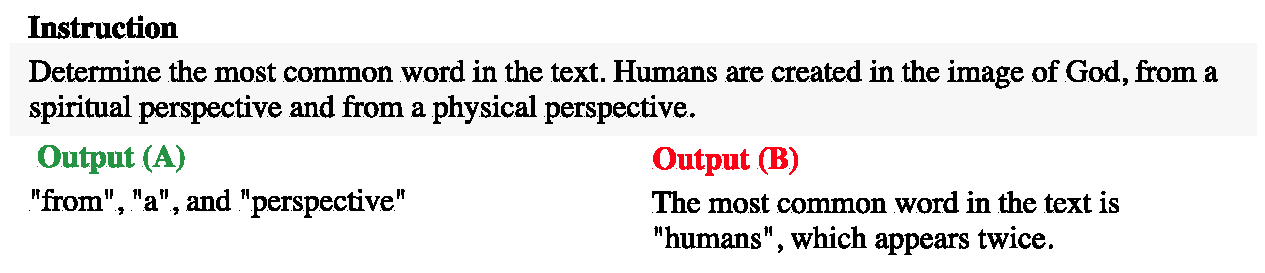
\includegraphics[width=0.9\textwidth]{figures/1.pdf}
  \caption{An instance from \llmbarnatural dataset. Output (A) is the gold preferred response.}
  \label{fig:appx_case_70b_data}
\end{figure*}

\begin{figure*}[t!]
  \centering
  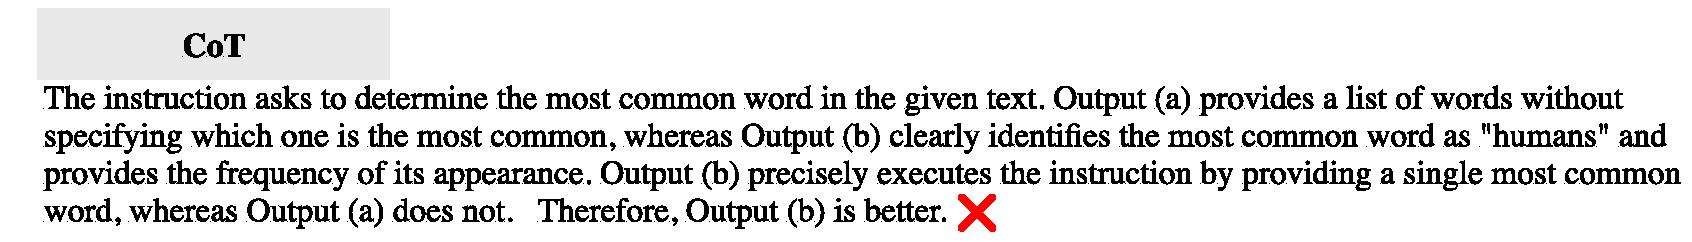
\includegraphics[width=1\textwidth]{figures/2.pdf}
  \caption{\llama-3-70b output under \texttt{cot} protocol.}
  \label{fig:appx_case_70b_cot}
\end{figure*}
\begin{figure*}[t!]
  \centering
  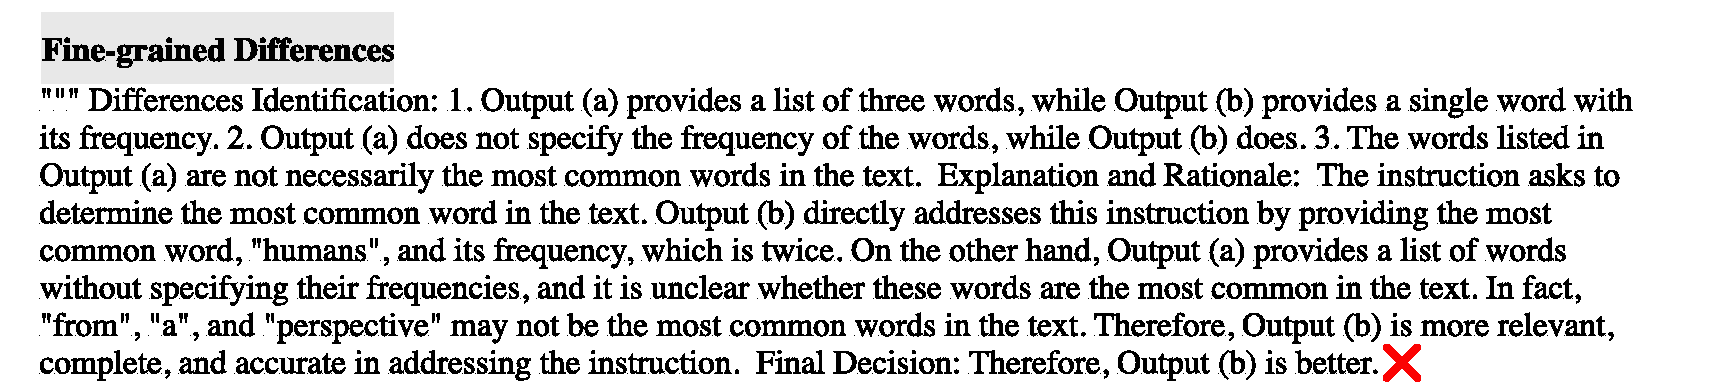
\includegraphics[width=1\textwidth]{figures/3.pdf}

  \caption{\llama-3-70b output under \texttt{fine-grained-diff} protocol.}
    \label{fig:appx_case_70b_fine}
\end{figure*}
\begin{figure*}[t!]
  \centering
  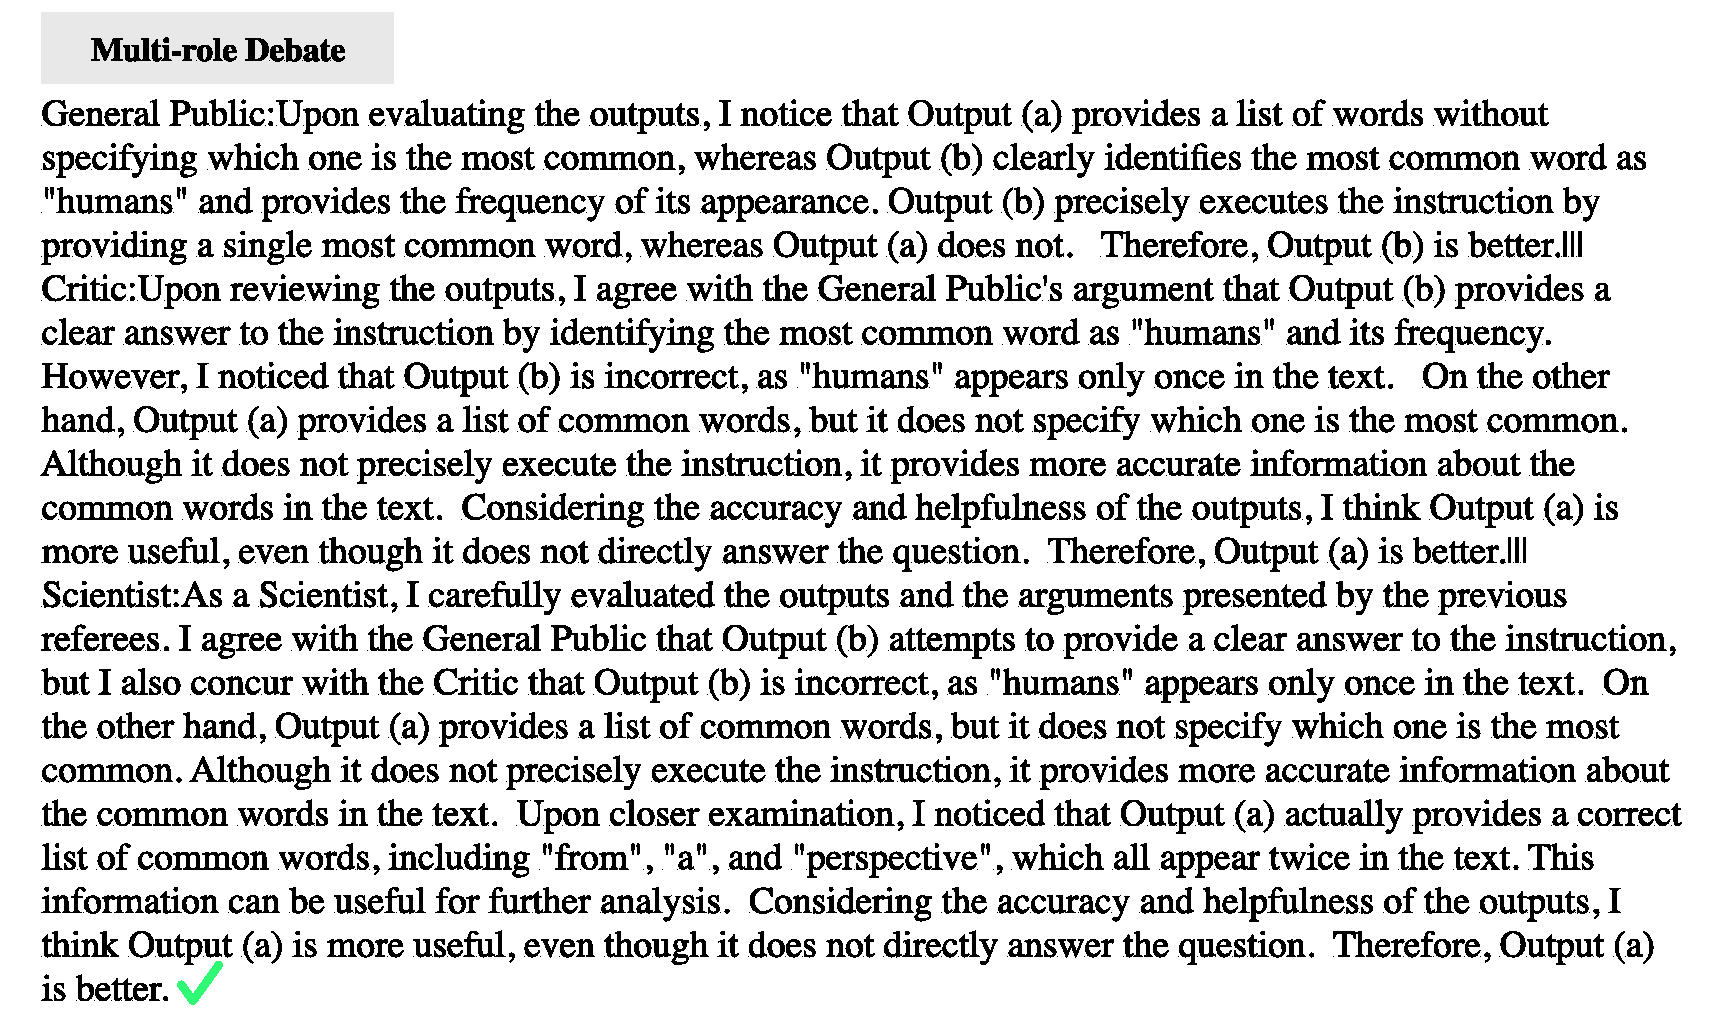
\includegraphics[width=1\textwidth]{figures/4.pdf}
  \caption{\llama-3-70b output under \texttt{multi-role-round2} protocol.}
  \label{fig:appx_case_70b_multi_role}
\end{figure*}


% 

% 

\begin{figure*}[t!]
  \centering
  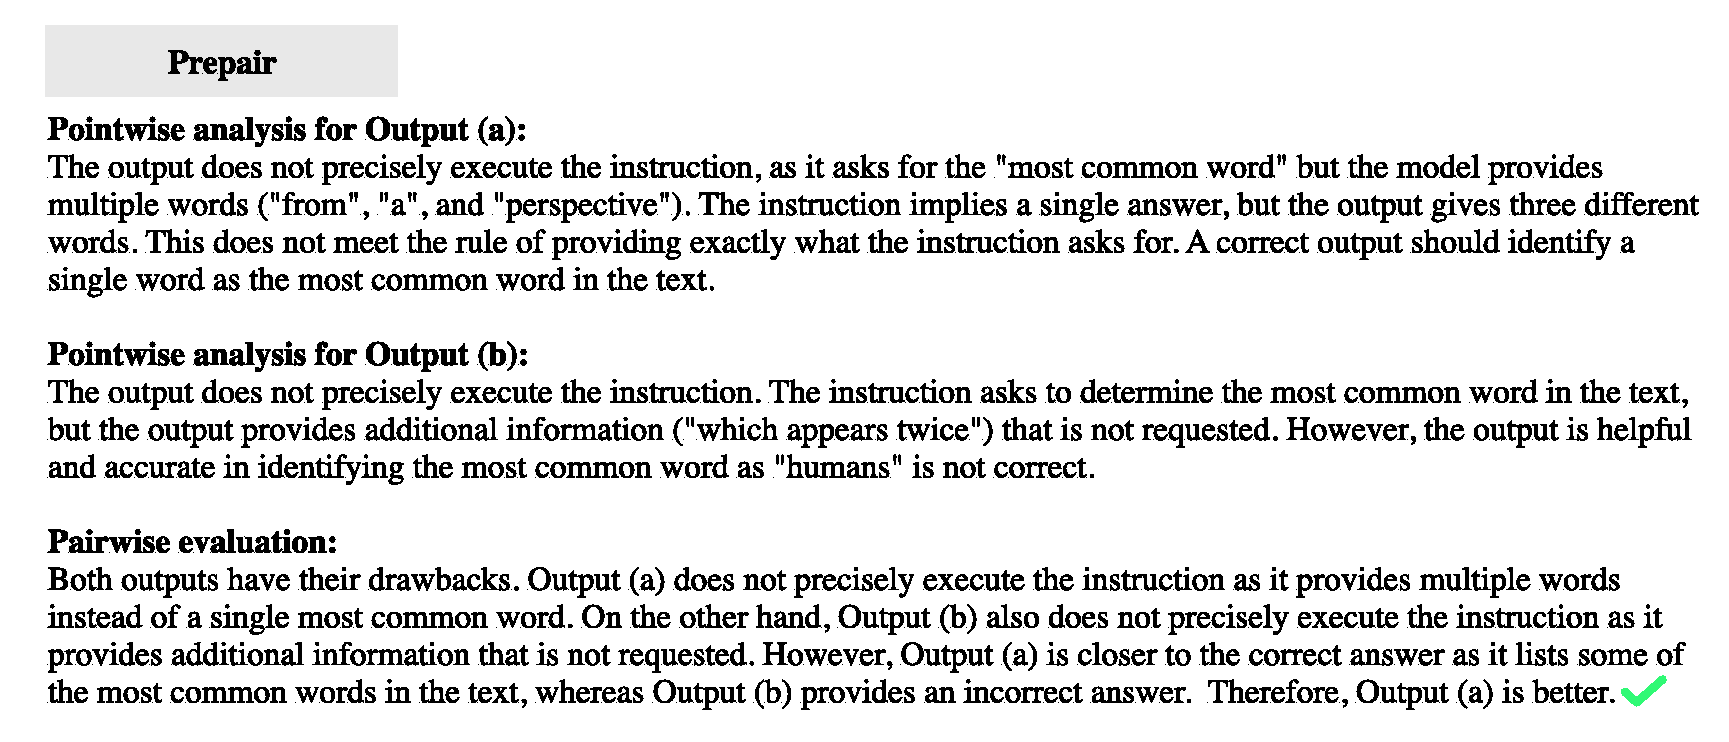
\includegraphics[width=1\textwidth]{figures/9.pdf}
  \caption{\llama-3-70b outputs under \texttt{prepair} protocol. Outputs from the pointwise analysis stage and the pairwise evaluation stage are presented.}
  \label{fig:appx_case_70b_prepair}

\end{figure*}

% 
